\title{The Adaptive Multi-scale Simulation Infrastructure - Design and Application}
\author{W.R. Tobin, V.W.L. Chan, M.S. Shephard}
\date{\today}
\documentclass[11pt]{article}
\bibliographystyle{siam}

\usepackage{amsfonts}
\usepackage{graphicx}
\usepackage{listings}
\usepackage{mathtools}
\usepackage{url}
\DeclarePairedDelimiter\ceil{\lceil}{\rceil}
\DeclarePairedDelimiter\floor{\lfloor}{\rfloor}

\lstset{basicstyle=\small,
        stringstyle=\ttfamily,
        frame=top, frame=bottom,
        captionpos=t}

\begin{document}
\maketitle

\begin{abstract}
\end{abstract}

\section{Introduction}\label{introduction}
[Need a couple sentences to talk about how multi-scale is important]
Implementation of multi-scale numerical simulations typically rely on either an ad-hoc set of algorithms designed for a particular problem, or on large frameworks and runtimes. 
Ad-hoc approaches, by their nature, are targeted to a particular multi-scale problem for a specific set of single-scale numerical codes, and thus offer no wider utility beyond their immediate usage as a simulation code.
Framework and runtime approaches are more flexible and admit a broader range of reuse, but typically necessitate that single-scale operations be adapted to work in the ecosystem they create.

Development of multi-scale simulations and methods to support the implementation of such simulations has been ongoing for several decades. 
Some approaches begin with the specification of multi-scale contributions during the specification of mathematical model.
However, multi-scale influences can be incorporated in a strictly numerical or computational sense, by combining implementations of established physical models operating at different scales referencing and effecting shared physical fields and values \cite{shenoy97} \cite{weinan2003heterogenous}. 

% classes of multi-scale problems
In order for a numerically multi-scale approach to be effective the domain associated with the scale of interest (the engineering scale) must be of sufficient size that conducting the entire simulation with terms and granularity orders of magnitude removed would make the simulation computationally intractable.
Thus some computationally reasonable subset of the engineering scale is assigned significantly finer scale(s) to simulate. 
The choice of location of supporting fine-scale simulations is largely dependent on the specific mathematical models and numerical methods used to implement the engineering scale simulation.
Two general classes of fine-scale simulation locality have been noted \cite{weinan2011principles}, 'A' type problems where local granularity requirements such as boundary layers or crack propagation necessitate use of localized fine-scale simulation, and 'B' type problems where fine-scale simulation is used to supplement or replace a continuum model at the engineering scale.
For either case the subset of the engineering-scale domain associated with finer scales are areas of the domain where the fine-scale contributions have the greatest impact on the evolution of the engineering scale simulation, in order to leverage the most utility from the multi-scale approach.

% types of numerical paradigms related to multi-scale, maybe mention that a problem using the concurrent multi-scale paradigm is discussed later in the paper?
Numerical multi-scale simulations fall broadly into two parallel paradigms, distinct from the choice of subdomain assigned to fine scale simulation.
In the sequential multi-scale paradigm, fine-scale computation is used to precompute quantities of interest for establishing an engineering-scale physical model, possibly using a lookup table or some other method to incorporate the multi-scale influences into the engineering scale \cite{weinan2011principles} \cite{garcia2008sequential}.
In the concurrent multi-scale paradigm, all scales are computed simultaneously and the required inter-scale coupling values are provided just-in-time \cite{weinan2011principles} \cite{zeng2010concurrent}.

% introduce scale-coupling topic to be discussed further in AMSI and methods sections
Numerically multi-scale simulations associate the computational implementations of single-scale physical models and cause them to interact by passing key physical terms between scales. 
This scale-coupling operation and may require the application of transformer functions to account for key physical differences between disparate scales. 
The primary purpose of such transformer functions is to convert physical coupling values produced by simulations operations at one scale to be meaningfully applied to simulation operations at the coupled, consuming scale. 
These transformer functions are typified by conversions between the unit metrics used by coupled scales. 
For example a micro-scale simulation will typically be implemented with units of $\mu$m while a macro-scale simulation might be implemented using units of cm.
Scale-coupling transformer functions may also be used for any additional coupling-term operations required to account for differences between coupled scales, such as dimensionalizing terms calculated in a dimensionless domain.

% introduce legacy component concept which should be discussed in AMSI and methods sections
Decades of numerical simulation development have resulted in a large and diverse array of widely used codes for single-scale simulations. 
This set of legacy codes represents a massive investment of development efforts, and thus leveraging the capabilities of such legacy codes for use in multi-scale simulations is desirable. 
Incorporating such codes into a functional numerical implementation of a multi-scale model has been a largely ad-hoc, per-code affair. 
Providing tools to ease the incorporation of legacy components into multi-scale simulations using general procedures while requiring minimal intervention in the legacy codebase results in less fracturing of the legacy codebases when incorporated into varied multi-scale simulations, and avoids the option of complete reimplementation of legacy code functionality in specialized multi-scale ad-hoc codes, or structured frameworks or runtimes.

Implementation of multi-scale simulations has fallen widely into two categories: purely ad-hoc implementations, and implementations supported by a structured framework or runtime. 
In the case of an ad-hoc implementation all support for multi-scale interaction is hard-coded into the simulation code itself. 
Frameworks and runtimes provide a robust set of scale-coupling operations, scale management,  and overall simulation management. 
The application programmer must tailor the numerical operations occurring at a discrete scale to operate using a set of interfaces or high-level modelling language required by the framework/runtime.
Ad-hoc implementations allow for overall optimizations at the cost of development time (and potentially complexity). 
Framework/runtime implementations often have a component-based approach that breaks the implementation of a simulation (single- or multi-scale) into discrete interoperable components. 
This approach requires that operations are implemented to work specifically within the set of interfaces understood by the framework/runtime.

\section{Adaptive Multi-scale Simulation Infrastructure}\label{AMSI}
The Adaptive Multi-scale Simulation Infrastructure (AMSI) is a set of libraries and tools developed by the Scientific Computation Research Center (SCOREC) at Rensselaer Polytechnic Institute. 
AMSI is designed to support the implementation and execution of dynamic concurrent multi-scale simulations on massively-parallel HPC machines.
AMSI provides support for several key operations needed for concurrent multi-scale simulations: modelling and managing scales, scale-coupling parallel communication, adaptively adding/removing scale-tasks, and load-balancing coupled scales. 
A key goal in the design and implementation of these operations is a focus on general applicability and avoiding adherence to specific interfaces.

The interfaces provided by the AMSI libraries are intended to facilitate the coupling of functional single-scale simulation codes.
This approach is used in order to mitigate development overhead associated with casting a simulation into a set of framework-specific components, or developing an entire ad-hoc set of multi-scale operations each time a new multi-scale code is being developed.
Several key multi-scale operations are planned and enacted by the AMSI libraries, allowing the application programmer (a programmer using the AMSI libraries to implement a new multi-scale code or interaction) to determine the most effective use of the tools provided. 
All interfaces are designed to be physics-agnostic, operating only on computational quantities with no meta-model of the relation between a coupling term and the mathematical derivation of the multi-scale interaction.

AMSI operates by maintaining a set of minimal simulation metadata in order to model various quantities of interest during simulation execution. 
AMSI provides mechanisms to assist in the implementation of run-time decision making and control decisions related to multi-scale execution, with a focus on allowing such adaptive procedures to be planned and implemented in a decentralized manner.
This design approach allows application developers to avoid centralized control decision bottlenecks.
Control decisions and associated parallel communication (as with most adaptive procedures) are best implemented at locations in code already requiring parallel barriers for synchronization.

In order to avoid the introduction of unnecessary parallel barriers into the code, AMSI control decisions are only  during operations which are already collective over the set of processes effected by a given control decision.

% need to expand this substantially
Frameworks and runtime systems have been developed which are intended for the development of specific multi-scale problems \cite{parker2006component} \cite{chopard2011framework} \cite{} and these frameworks have in some cases been expanded to facilitate the implementation of additional multi-scale problems \cite{berzins2010uintah}.

Such systems require that the application developer cast the problem of interest into a set of predefined components (interfaces, tasks, etc.) or specify the problem through a high-level modelling language in order to take full advantage the services provided by the framework. 
Leveraging a component-based design is valuable from a software engineering perspective, as it allows composition of disparate components into a cohesive application. 
This approach also introduces new complexities involved in defining the set of components and how they interoperate in the framework, shifting some complexity up the abstraction hierarchy.
The core features of AMSI used for multi-scale simulation management and communication are provided with no requirements of adherence to a specific component definition.

Typically simulation flow control is determined solely by a runtime system. 
A framework may also limit specific features of the numerical implementation to those provided by the framework. 
This includes domain discretization models and associated adaptive processes -- structured and unstructured meshing and associated refinement algorithms, particle-in-cell methods, etc. -- convergence algorithms for both the minimization of the relevant residuals (Newton-Raphson, etc.) as well as iterative solution of the resulting linear system (KSP, GMRES, ILU, etc.).

AMSI supplies several numerical components consisting of an adaptive finite element system, linear algebraic solver, and nonlinear convergence operators available as both simple C++ class interface definitions, as well as implementations of these interfaces built on top of other software supplied by SCOREC \cite{core} for finite element analysis operations, Simmetrix mesh database software \cite{simmetrix}, and the PETSc linear algebraic solver \cite{petsc-web-page} \cite{petsc-user-ref} \cite{petsc-efficient}. 
Usage of the supplied numerical components is not required to make use of the multi-scale capabilities of the AMSI libraries, but provide a jumping-off point for application developers needing to implement a new single-scale code to incorporate into a multi-scale simulation.

Implementing required numerical operations inside an existing framework is of course possible, though it may prove an additional -- undesirable overhead for an application programmer interested only in utilizing the multi-scale framework to implement a simulation, rather than implementing the various numerical operations often optimized in widely available packages and libraries.

\section{Methods}\label{methods}

\subsection{Simulation Construction with AMSI}
In order to construct a multi-scale simulation using the AMSI libraries the following must be specified: the Scales in the problem, the ScaleCouplings between individual scales, the DataDistribution of coupling data produced by each Scale in a coupling, and the CouplingPattern used to communicate coupling data during coupling operations. 

A Scale is a data structure modelling the parallel state of a discrete simulation scale and all operations (or tasks) occurring at that scale. 
All Scales have a set of MPI\_Ranks associated with them through an intermediary structure called the RankSet. 
In the current implementation the RankSet of any two Scales in a simulation must be non-overlapping.  
A Scale is required for the specification of all other data structures in the AMSI libraries. 

A ScaleCoupling is an object denoting that scale-coupling communication will take place between two scales at some point during the simulation. 
All interacting Scales in a simulation must declare a ScaleCoupling between them.
For generality the ScaleCoupling relationship is non-commutative, thus Scale A is related to Scale B if and only if A produces coupling data which will be sent to B.
Symmetrical coupling relations therefore require two ScaleCouplings, one denoting the production of data by A for consumption by B and one denoting the reverse.
Scales not related through a ScaleCoupling cannot create CouplingPatterns which are required for multi-scale communication and therefore cannot pass scale-coupling data through the AMSI libraries.

A DataDistribution is a structure denoting the parallel distribution of terms produced by a scale for use in a ScaleCoupling relationship for a specific CouplingPattern. 
The DataDistribution is minimally described as a parallel array of integers on the RankSet associated with some Scale A, thus the length of the array is $|A|$ (the cardinality of the RankSet currently assigned to Scale A).
The DataDistribution may be dynamically modified during the simulation to reflect single-scale adaptive procedures or specifically multi-scale adaptive features (such as selectively adding/removing specific fine-scale simulations). 
Each Scale may have many DataDistributions, and a DataDistribution is not tied to a particular ScaleCoupling, in the event that the same distribution characterizes the scale-coupling data produced by a Scale needed by multiple coupled scales.

A CouplingPattern describes the parallel communication required to send scale-coupling data produced by the the sending Scale in a ScaleCoupling and described by a DataDistribution. 
A CouplingPattern based on the ScaleCoupling of scale $A$ coupled to scale $B$ is described most simply as a matrix $C \in \mathbb{N}^{|A|\times|B|}$ (where $|X|$ is the cardinality of the RankSet currently assigned to scale X). 
The quantity $C_{ij}$ represents the quantity of scale-coupling terms (of arbitrary type) to be sent from process $i$ in the process set assigned to $A$ to process $j$ in the process set assigned to $B$.
As the DataDistribution upon which the CouplingPattern is based is allowed to change due to adaptive procedures, all CouplingPatterns related to a DataDistribution are updated when adding/removing terms from a DataDistribution. 
Finalization of the creation of a CouplingPattern causes the creation of a DataDistribution on the receiving Scale, as modifications to a DataDistribution may happen on either side of the ScaleCoupling, but the initial CouplingPattern must be created by the producing Scale.
Determination of how a CouplingPattern should change based on changes to the underlying DataDistribution may differ for potentially each multi-scale use-case, so hooks are provided so the application program may correctly update CouplingPatterns for their specific use case.
As both Scales in the ScaleCoupling must know about the modification in order to appropriately handle the modified scale-coupling data being communicated, all modifications to the CouplingPattern and DataDistribution are communicated from the producing Scale to the consuming Scale. 
Due to this requirement it is best to update DataDistributions completely in a single operation following any adaptive procedures, since these are often parallel barriers already.
Similar operations are provided for scale-sensitive load-balancing operations taking place on a sending or receiving scale in a ScaleCoupling, as the associated scale must be informed of the changes to the relevant DataDistribution.

ScaleCoupling transformation functions are not currently supported by the AMSI libraries and must be implemented by the application programmer for the each specific multi-scale interaction.

\subsection{Parallel Operations}\label{paralle_ops}

Each Scale in AMSI represents some number of individual scale-tasks. 
Scale-tasks are not an AMSI construct, merely an abstraction to allow grouping of multiple copies of the same single-scale simulation into a single Scale. 
Minimally a Scale possess a single scale-task. 
For example the biotissue simulation (discussed in Section \ref{biotissue}) the Macro Scale has a single scale-task, a parallelized finite element analysis simulation.
However a Scale may also possess many scale-tasks, each a duplicate of a single-scale simulation.
Again in the biotissue example case, the Micro\_FO Scale has a number of scale-tasks (individual Representative Volume Element (RVE) simulations) related to the number of Macro mesh elements.
The management of these scale-tasks the responsibility of the application programmer, though changes made that redistributed terms modelled in any DataDistributions should be noted and used to update appropriately once dynamic/adaptive operations have ceased. 
Adding/removing terms from a DataDistribution may result in the requirement that scale-tasks be instantiated/deleted to accommodate the modification.

When DataDistributions are modified the modifications must be reflected across the RankSet associated with the Scale on which the DataDistribution is defined. 
This procedure is called Assembly, where each rank contributes the local (and hence valid) portion of the control data to arrive at a valid Scale-global value.
In practice this reduces to an MPI\_Allgather operation for the DataDistribution, but for other types of AMSI control data (most specifically the CouplingPattern) the implementation of the Assembly operation requires additional operations. 

When CouplingPatterns are modified (as a result of a changing DataDistribution) the Scale informing the modification must also ensure that the coupled Scale receives the corrected CouplingPattern. 
This process is called Reconciliation, and has two phases the inter-scale phase and the local-scale phase.
In the inter-scale phase a sparse representation of the relevant CouplingPattern data (relevant meaning related to the rank receiving the data, informing that rank fully of only the role it plays in the communication) is communicated from the modifying scale to the modified scale. 
In the scale-local phase a specialized Assembly operation is performed on the received partial updates to update the full CouplingPattern representation on all processes in the modified Scale.

%% revised up to here, with sporadic edits after

All communication and planning operations in the AMSI libraries use an implicit local numbering for data distribution terms, the index associated with the term in a local serialized buffer. 
Usage only of implicit ordering was decided upon in order to reduce the memory impact as the simulation scales, as any meta-data which scales with the simulation will necessarily pose a memory issue once scaling hits some threshold.

Since scale-tasks are an abstraction the AMSI systems cannot provide direct operations on scale-tasks, but provide mechanisms for the application to inform AMSI of such operations when they occur.

Additionally, scale-tasks associated with specific subsets of a process set (either a single process or several processes) may be migrated in part or in whole. Migrating a scale-task in part amounts to using load balancing facilities on the associated processes to redistribute all data scale-task from a scale-task to a subset of the previously associated processes, allowing the freed processes to be assigned data from other scale-tasks. Migrating a scale task in whole constitutes using load balancing operations on the process set associated with the entire scale to move all pertinent data between subset of the managed process set. AMSI provides operations to enact load-balancing operations from plans such as those generated by Zoltan algorithms.  In the current implementation these operations are collective on the process set associated with the managed scale.

While the primary scale (the scale associated with producing the solution for the overall simulation) is often thought of as controlling the tertiary scales in terms of dynamic instantiation, this is not assumed in the AMSI implementation. Any scale is capable of informing the process set associated with a coupled scale of the addition or deletion of individual scale-tasks. At present it is dependent on the developer to implement the capability of a scale to accept additional scale-tasks.

Scale-coupling communication is guided by data distributions and communication patterns. A data distribution is a representation of individual units of scale-coupling data distributed across a single scale-task. The format of the coupling data is arbitrary (so long as it can be serialized and provided for use by MPI communication primitives). A data distribution represents the smallest unit of data important to the scale-coupling communication, which is necessarily distinct for various multi-scale use cases.

Scale-linking quantities are dynamically registered with the AMSI system using a data distribution defined on a scale by the scale-tasks operating at that scale. Production of a communication pattern is required prior to executing a scale-coupling communication, and the pattern must be reconciled (synchronized across the coupling relationship) prior to being used to guide a coupling communication operation (and when the communication pattern is altered by the scale providing the coupling data). Several simple communication pattern production algorithms are provided by AMSI, but these are relatively trivial due to the nature of scale-coupling communications and the general nature of the AMSI libraries. Hooks are provided for users to implement algorithms for the construction of communication patterns tailored to the specifics of their problem.

At present an application developer must implement up-/down-scaling operations required for their particular multi-scale use case, hooks will be provided in future releases to automate application of such operations during scale-coupling. The current implementation includes blocking versions of the scale-coupling communication operations. Asynchronous versions have been designed but are not currently implemented due to lack of immediate need in the primary AMSI use case.

\section{Soft Tissue Simulation}\label{biotissue}
The Biotissue code is a multi-scale simulation of soft organic tissues, consisting of an engineering-scale simulation using the finite element method, and a micro-scale quasistatics force-balance simulation. The Cauchy Momentum Balance Equation for a body in static equilibrium is used as the governing equation for the macro-scale simulation.
%
\begin{align}
\nabla \cdot \pmb{\sigma} =& \; 0 \text{ in } \Omega \label{momentum_balance} \nonumber \\
\pmb{\sigma} \cdot \pmb{n} =& \; \pmb{t} \text{ on } \partial \Omega \nonumber
\end{align}
%
Specific quantities needed to compute the elemental tangent stiffness matrices and force vectors are instead supplied by the micro-scale force-balance simulations, which occur at each numerical integration point in the engineering-scale mesh \ref{biotissue_hierarchy}.
%
\begin{figure}
  \begin{center}
    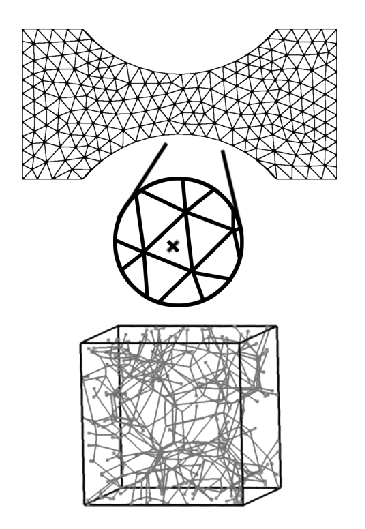
\includegraphics[height=2in]{biotissue_visual_hierarchy.eps}
  \end{center}
  \caption{\small biotissue multi-scale problem}
  \label{biotissue_hierarchy}
\end{figure}
%

The incremental displacements (deltas generated by the previous Newton-Raphson iteration) on each engineering-scale finite element node are used to distort the a dimensionless representative volume element (RVE) through a dimensionalized abstraction of the RVE embedded in the engineering domain and an associated displacement mapping term $\frac{d\mathbf{RVE}}{d\mathbf{FE}}$, the first order relation between the incremental displacement of an RVE with respect to the displacement of the associated mesh element. This results in each micro-scale node being displaced. Each RVE is a dimensionless unit cube containing a connected collagen fiber network, for the present results the fibers are implemented as truss elements and their distribution is generated using Delauney triangulation, resulting in a high coordination number at each node and consequently a numerically stable fiber network. The micro-scale boundary condition necessitates that the force exerted by each fiber network node located on the boundary of the RVE be zero. The micro-scale global Jacobian is formulated along with the force vector, wherein the boundary condition is enforced by setting specific rows of the force vector associated with boundary nodes to zero.

Another Newton-Raphson iterative process occurs at micro-scale to converge to the set of displacements resulting in force equilibrium for all the fibers within the fiber network constituting the RVE. After a micro-scale simulation converges to a solution, the Jacobian and force vector are then evaluated again at the solution position, the force exerted along the boundary of the RVE is summed for each of the principal and shear components of a stress tensor, which is then dimensionalized and sent back to the engineering-scale for use in the elemental tangent stiffness matrix formulation. More detail into the derivation of this multi-scale system can be found in \cite{stylianopoulos2008thesis} \cite{agoram2001coupled} \cite{stylianopoulos2007multiscale} . Discussion of the dimensionalization of the dimensionless force terms produced by each fiber network can be found in \cite{stylianopoulos2007volume} \cite{chandran2007deterministic}.

The simulation two nested Newton-Raphson operations occurring; during each macro-scale Newton iteration every micro-scale RVE must undergo a full Newton-Raphson convergence process.

\section{Results and Discussion}\label{results}
The biotissue simulation was run on the AMOS BG/Q machine housed at the CCI facilities. Both strong and weak scaling studies were conducted up to an eighth of the total machine core count, or 16384 cores. The ratio of macro-scale to micro-scale assigned processes was held at 1:127, and the total core count was kept as an integer power of 2 in order for the SLURM job scheduler to submit the jobs to the compute nodes in a timely manner. The precise calculation used to determine macro and micro process counts is given by
%
\begin{lstlisting}[language=Bash,caption={process assignment calculation}]
  NP=$(( $NUM_MACRO * 128))
  NUM_MICRO=$(( $NP - $NUM_MACRO))
\end{lstlisting}
\label{macro micro ratio}
%

Separate timings were taken for various sections of the simulation code, isolating the micro-scale computation, macro-scale linear system assembly and calculation of elemental linear systems, and macro-scale linear system solution. In addition, the time for spent in the AMSI subroutines for communication was also measured. Thus the behavior of each section of the code is independently evaluated in our scaling study, as well as the overall execution time.

%
\begin{figure}
  \begin{center}
    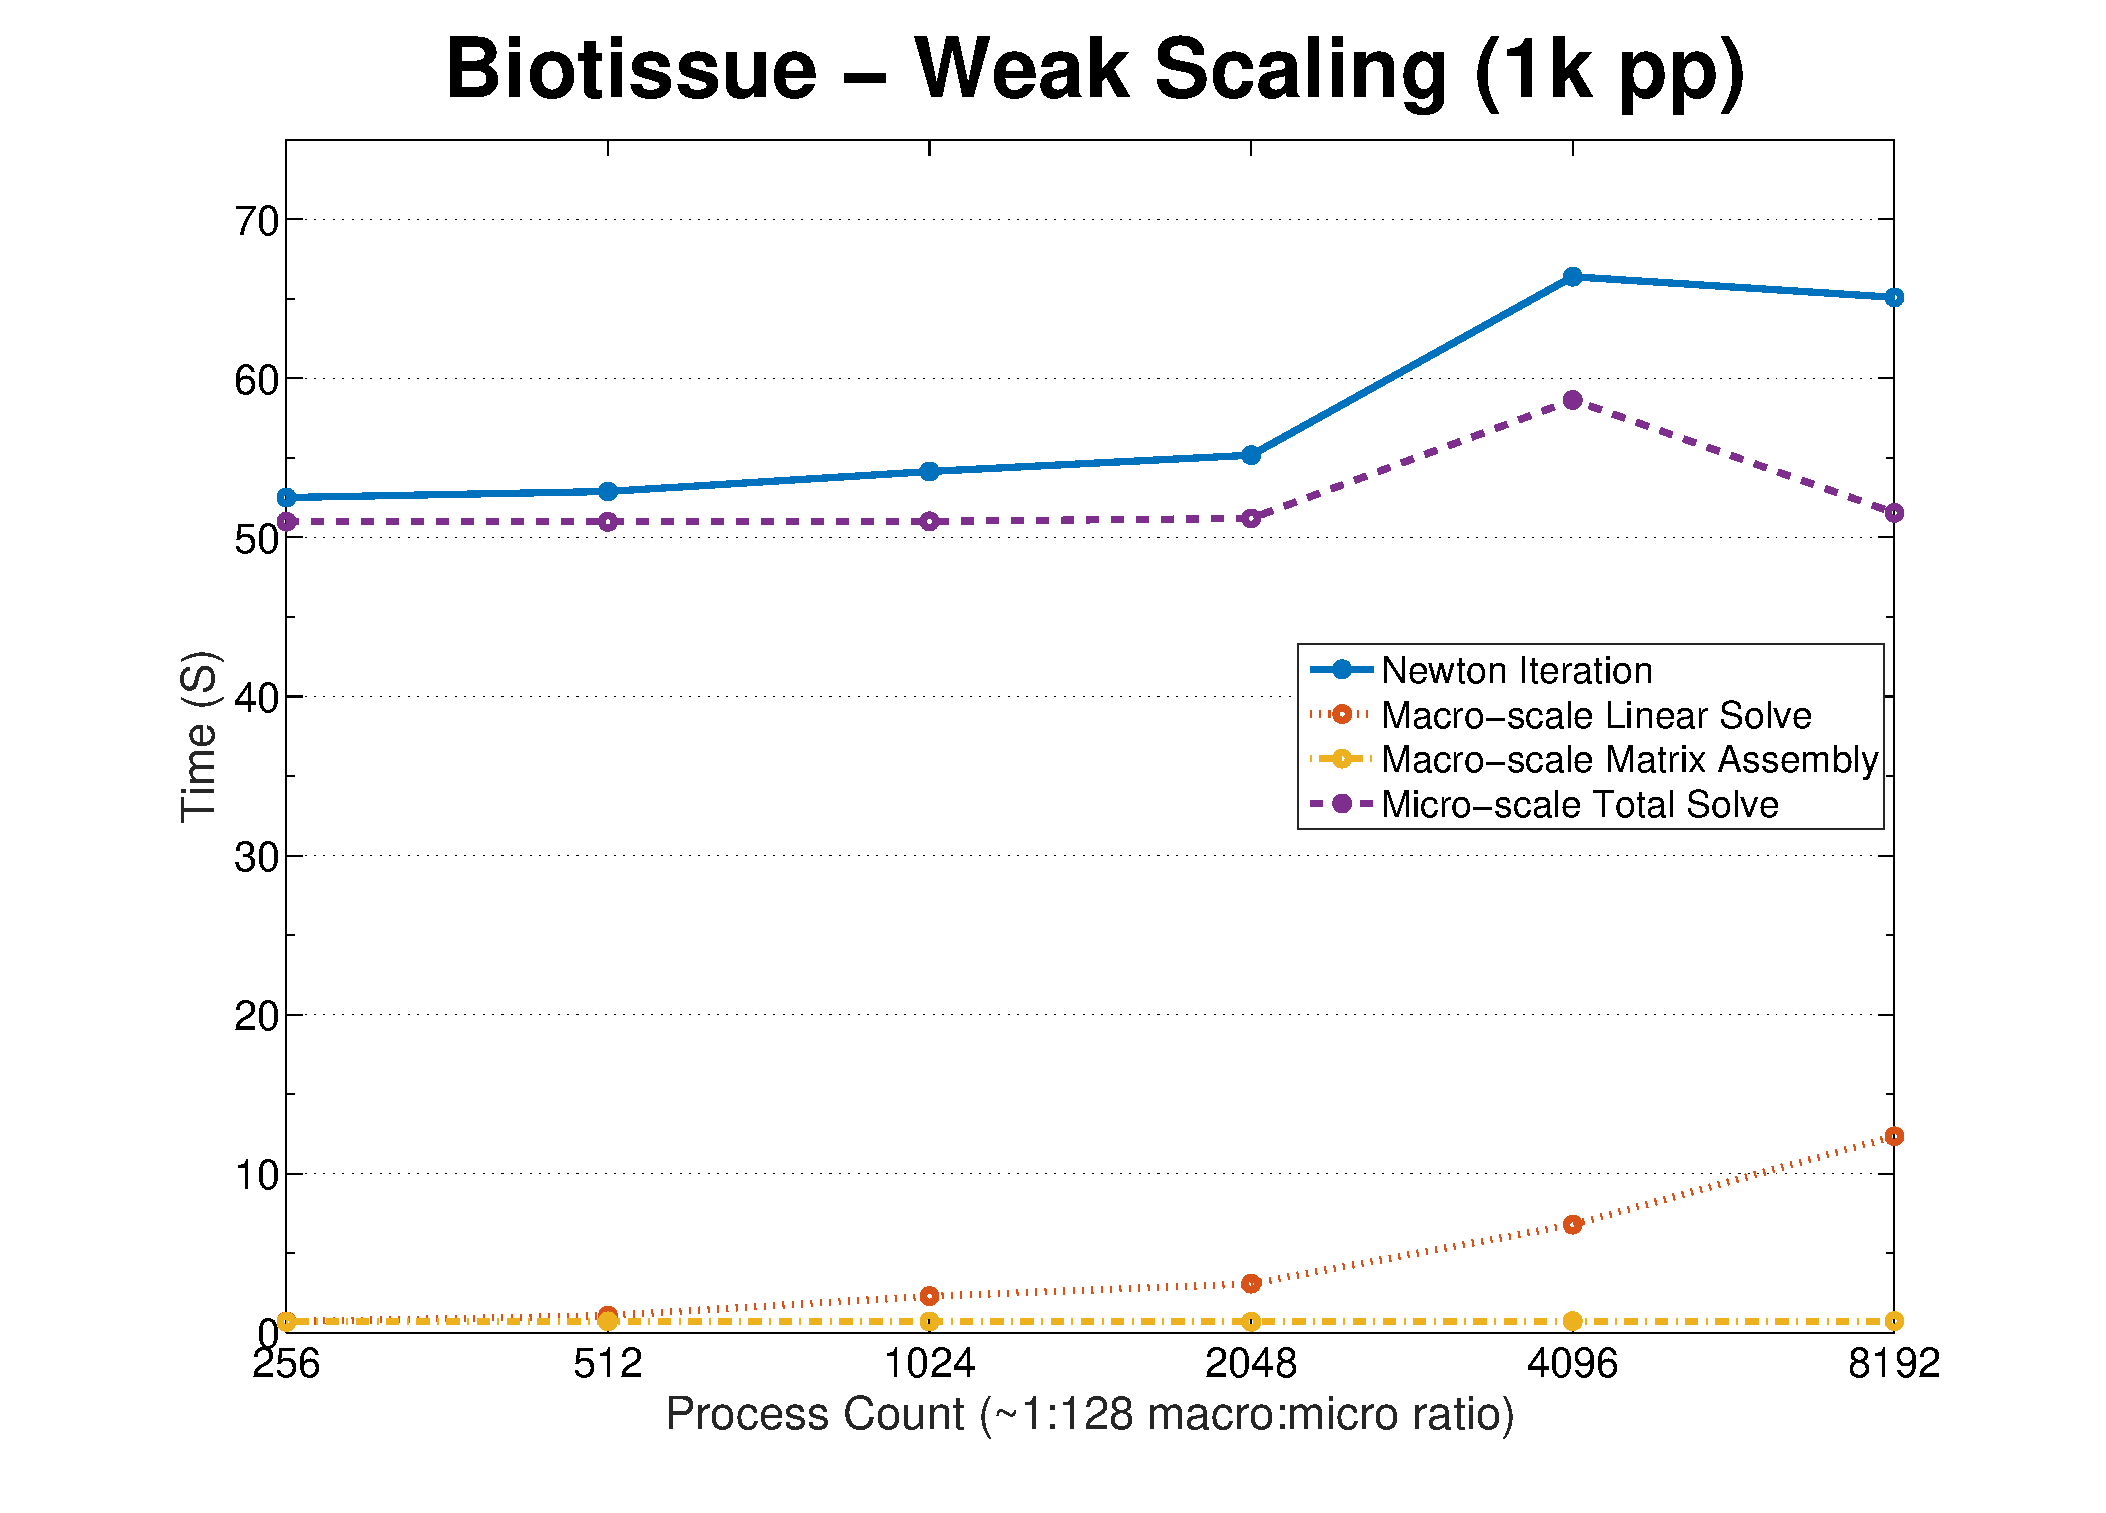
\includegraphics[height=2in]{ws_phil.eps}
  \end{center}
  \caption{\small weak scaling}
  \label{weak scaling}
\end{figure}
%
Keeping the work per process approximately constant (1k elements per macro-scale process, with the 1:127 macro-micro ratio as specified in listing \ref{macro micro ratio}) it can be seen that the time to compute every RVE in the system stays relatively consistent, while the time to solve the macro-scale linear system increases, causing a modest increase in the overall time per macro-scale Newton iteration.

%
\begin{figure}
  \begin{center}
    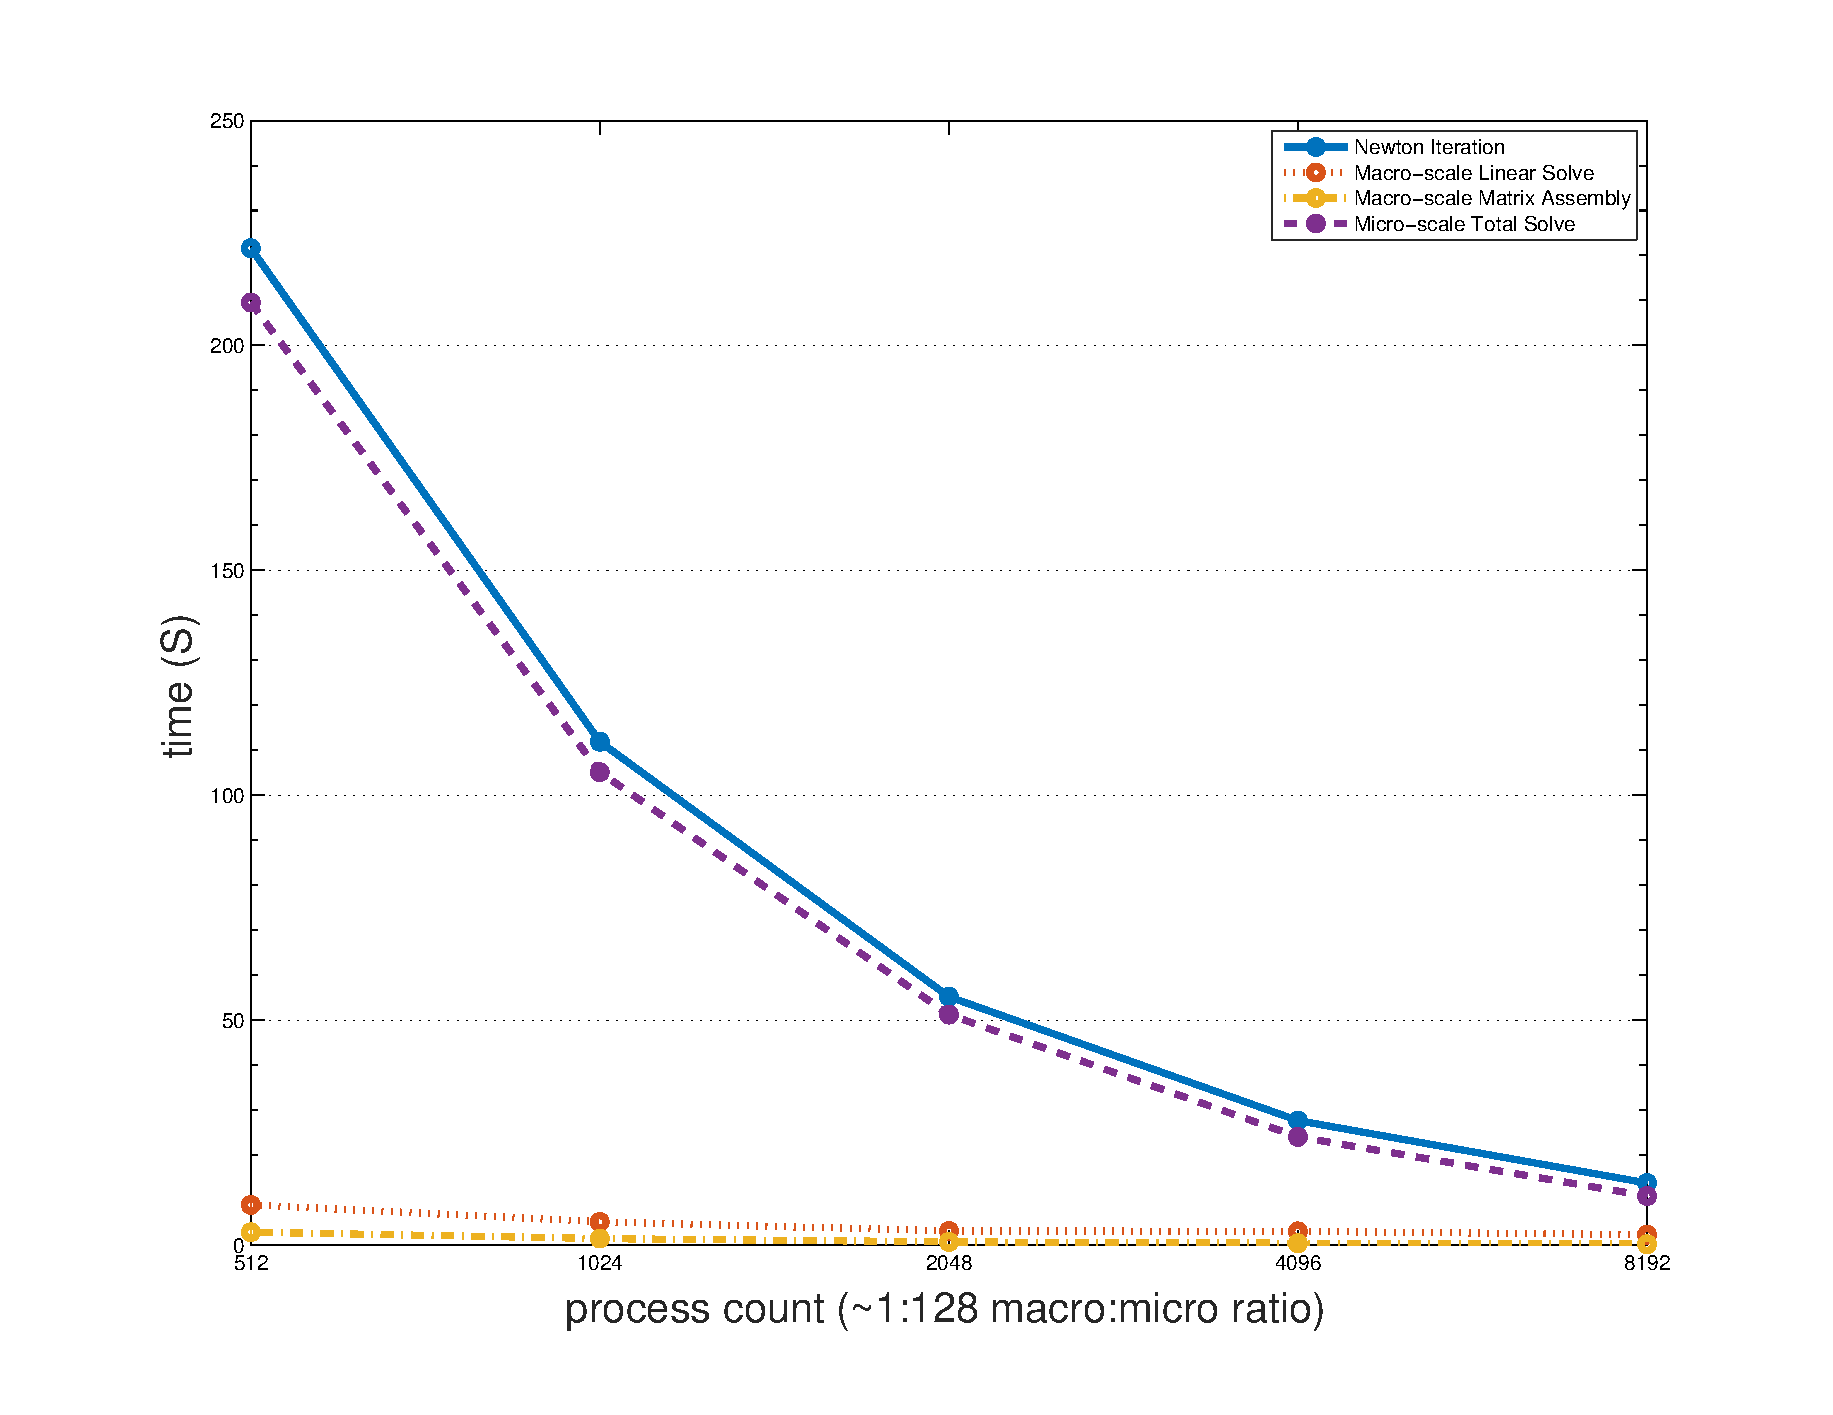
\includegraphics[height=2in]{ss_phil.eps}
  \end{center}
  \caption{\small strong scaling}
  \label{strong scaling}
\end{figure}
%
As the problem size is held constant with respect to the number of individual elements in the engineering scale domain discretization the simulation displays near optimal convergence to the macro-scale solve time alone, which is also reducing in time cost. The limiting factor in the speedup of the overall simulation is the potential speedup of the macro-scale simulation rather than the micro-scale simulation with fiber-only RVEs. As indicated in the weak scaling results this is related primarily to the macro-scale linear solve communication time increasing. At present an incomplete LU factorization is used to solve the linear system formulated at macro-scale each Newton iteraion (using PETSc configured with the superLU\_dist solver \cite{li05superlu} \cite{lishao10superluilu} \cite{lidemmel03superludist} ). Using instead an iterative solution method to reach a desired level of accuracy may result in stronger scaling at macro-scale, but as yet this approach has been unneeded due to the preponderance of time spent computing micro-scale results in use cases.

Many problems of interest will possess finite elements numbered in the tens to hundreds of millions of degrees of freedom, such that a suitable partitioning of the mesh to cores on the machine in terms of elements per partition (and directly the macro-scale time-to-solution) may require a substantial fraction of the total cores on the machine for macro-scale to execute in reasonable time. AMSI provides services for dynamically adding and removing individual scale-tasks to a specific scale, which can be utilized to limit RVE usage to only those locations in the multi-scale mesh most influential on the overall evolution of the simulation.

AMSI-specific results of some sort...?

Could include utilization/idle time metrics, but those are far more relevant to the load balancing paper...

\section{Conclusions and Future Work}\label{future_work}

The Adaptive Multi-scale Simulation Infrastructure provides a valuable set of tools to facilitate the implementation and execution of multi-scale simulations without imposing restrictions on the application developer. Usage of the core operations of the AMSI libraries does not require adherence to a specific set of interfaces nor usage of an abstract modeling language, which complicate inclusion of legacy components into multi-scale simulations.

Scale-sensitive load-balancing operations have been developed for the biotissue multi-scale test problem. Unfortunately the problem does not exhibit load persistence in the current parallel execution space task discretization, so an alternative parallel discretization such as overdecomposition with work-stealing to enforce more local balancing operations and occasional global balancing operations is being explored.

Development of libraries concerned with higher levels of abstraction of the multi-scale problem will also be valuable in easing the development of new multi-scale simulations from the perspective of the application programmer. High level abstractions such as the Scale Separation Map in \cite{chopard2011framework} could provide mechanisms to provide initial configuration information to the AMSI system during the initialization phase, as well as assist in the implementation of (or usage of existing library-provided) up-/down-scaling operations.

An RVE simulation taking into account inter-fibril matrix material has been developed \cite{lake2012mechanics} \cite{zhang2013cross} \cite{zhang2013coupled}. This alternative RVE will be incorporated into the multi-scale model as an alternative to the fiber-only RVE, to be used in areas of the macro-scale domain determined to be most critical to the overall evolution of the global system, or where error accumulation through model inaccuracy is to be minimized. As this fiber-matrix RVE represents a more significant source of computational complexity, it is independently parallelized -- in contrast to the fiber-only RVE -- and will represent a compelling use case for the parallel execution space discretization and scale-coupling communication management capabilities of the AMSI libraries.
\bibliography{citations}

\end{document}
